\subsubsection{Modelo \acrfull{ar}}\label{model_ar}


Un modelo \acrshort{ar} es otro tipo de redes neuronal recurrente. Esta red tiene como peculiaridad que el resultado obtenido se usa como valor de entrada para el calculo de la siguiente iteración. El modelo generado gráficamente es el siguiente:
\begin{figure}[H]
    \centering
    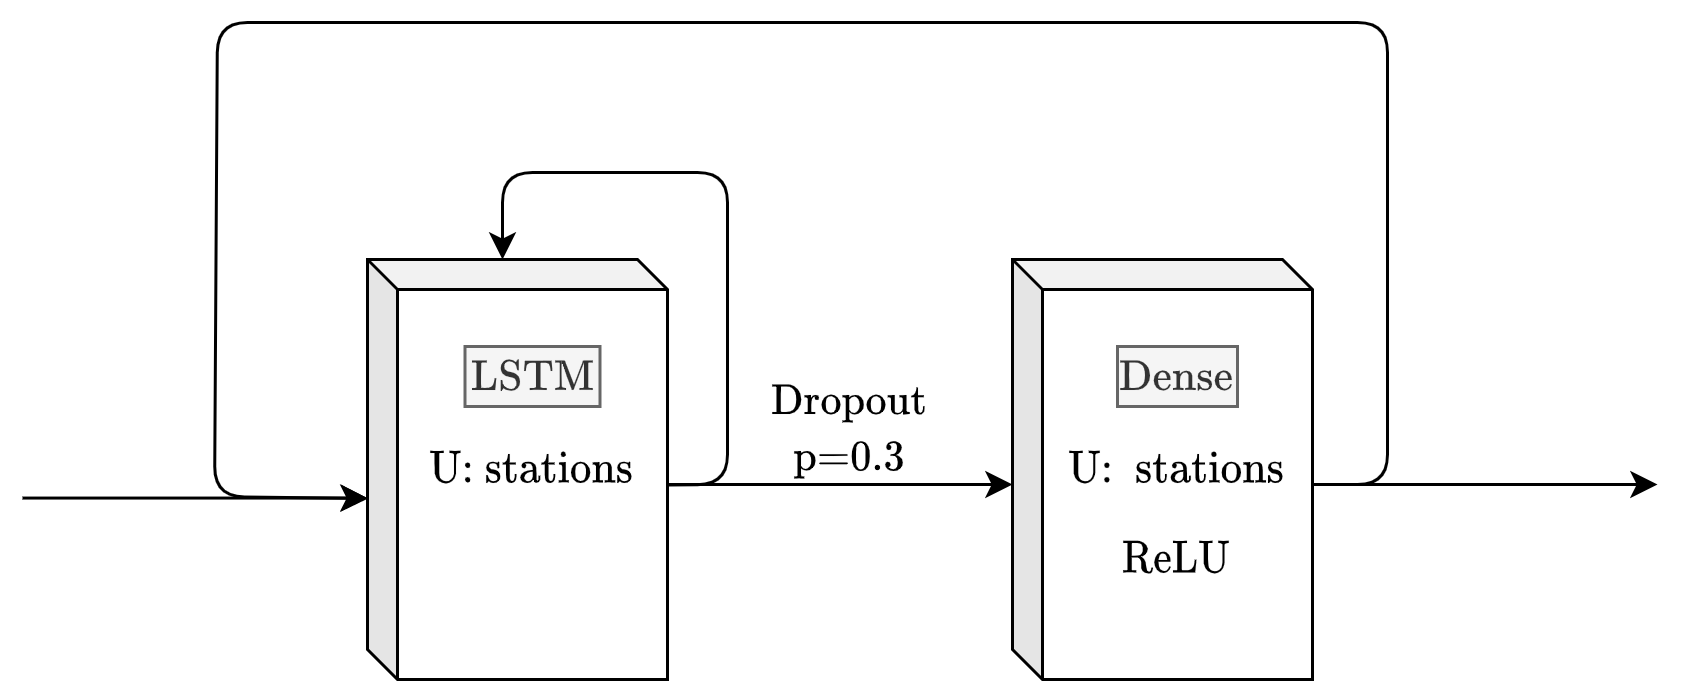
\includegraphics[width=10cm]{images/solution/models/AR.png}
    \caption{Modelo recurrente \acrshort{ar}}
    \label{fig:dense-model}
\end{figure}

El modelo tiene una capa \acrshort{lstm} junto con una capa densa. La salida de esta capa que es la predicción del modelo se reintroduce en el modelo para predecir el resto de predicciones.
\newline

\textit{Tensorflow} no dispone de un modelo en su librería herramientas que supliese las necesidades que se buscaban y por esa razón, se ha tenido que implementar este modelo usando otra técnica. Se ha creado una clase nueva que hereda de \small\verb|tf.keras.Model| y la cual tiene tres métodos: \small\verb|__init__|, \small\verb|warmup| y \small\verb|call|. De esta forma se pueden generar modelos que puedan tener arquitecturas singulares y distintas a las \textit{pass-forward}. Para la implementación se ha seguido la documentación de \textit{Tensorflow} \cite{tensorflow2015-whitepaper} y \textit{Keras} \cite{keras}. El código desarrollado para esta clase se puede leer en el Apéndice \ref{app:ar}.
\newline


Para crear un nuevo modelo \acrshort{ar} simplemente se genera una nueva instancia de la siguiente manera:
\begin{minted}[fontsize=\scriptsize]{python}
AutoRegressive(lstm_units=stations, steps=steps, stations=stations)
\end{minted}

Los resultados del modelo se pueden ver junto al resto de resultados en la sección \ref{results}.